\chapter{Network Management} \label{chap:nm} %% chapter 3

\par This chapter focuses on the management of networks, where we explore what is most necessary to obtain a comprehensive understanding of the network; formalize the statistics that can be reported via OpenFlow; see some 
research that has been done in the management of SDN applications, including what existing controllers provide us; and finally explore the way that DDoS detection and mitigation is usually implemented.

\section {Introduction}

\par As networks grow larger and more complex, systems must be put in place that allow for closely monitoring the resources that make up the network, while also allowing for a certain freedom for the possible constant change of the 
network. As such, typical vendor solutions don't really fit into this ever changing landscape, since they present very solid and vertically integrated solutions. The SDN paradigm, however, is able to solve this issue, since it 
enables for the centralized control of the underlying networks, which provides visibility and even control over the network, simplifying network diagnosis or troubleshooting. 
\par Although SDN is a promising paradigm in terms of networking management, it also introduces some points of failure that are non existing, or not as impactful in current networking deployments. This is related, for example,
to the centralization of the controller, which makes it susceptible to Denial-of-Service attacks or even the possibility of some malicious attacker that could possibly exploit the privileged view that the SDN controller has.
\par The topic of network management is very extensive, due to the several components that make up today's networks, and the vast amount of information that they provide. It can be summed up as the operation and maintenance 
of network infrastructure so that the service it provides is not only "healthy", but also is operated at a level that keeps costs down for service providers. 

\section {Requirements for management systems}

\par As the complexity of the networks, and network devices that compose them grow bigger and bigger, the management systems should accommodate for the their necessities. As such, the basic groups of requirements for management 
functions are that defined in the ITU-T X 700 Recommendation \cite {CITE - ITU T Recomendation} are:

\begin {itemize}
    \item \textbf {Fault management} is the capability for detection, isolation and correction of abnormal operation in the system
    \item \textbf {Accounting management} provides ways to monitor the system resource utilization, and using this data to generate information about the costs that the operation of a certain resource will incur. This 
        allows for better optimizing the network utilization of network, as it provides insights on how to plan the evolution of the network
    \item \textbf {Configuration management} is related to the maintenance and updates of hardware and software in the network, and the general setup of devices that allow to start, maintain and terminate services 
    \item \textbf {Performance management} relates to monitor systems for the traffic utilization, response time, performance and logging histories. This allows to maintain Service Level Agreements (SLA) from the service
        provider and the client, providing better services even in cases of unusual traffic.
    \item \textbf {Security management} enables setting up security policies in terms of access control to resources, private information protection, among others.
\end {itemize}


\par A network management system usually consists of a centralized station, and management agents running on the network devices. Using management protocols, the agents can report to the station information about the its operational 
status, which includes information ranging from CPU load to bandwith usage. Typically this information can be retrieved by the controller polling the agents, or the agents sending information on their own, usually to inform
status changes. Using this information, the network operator can get insight on the performance or possible errors of the devices that are monitored. In the next section, we explore one of the most popular management protocols,
SNMP.

\section {SNMP}

The Simple Network Management Protocol is an IETF defined protocol that allows for the interconnection of networking devices, and provide a structured way to retrieve relevant information about these devices. As the name suggests,
SNMP allows for a simplified approach to network monitoring, since it reduces the complexity of the functions that the management agent needs to comply with, which bring several advantages, like reducing
the costs for development of management tools; provides a way to monitor, independently from different hardware providers the resources; and also supports freedom in extending the protocol in order to include other aspects of 
network operation. \cite{CITE - RFC 1157} %% XXX cite https://tools.ietf.org/html/rfc1157
\par  The architectural model of SNMP can be described in figure \ref{fig:snmp}.
    
\begin{figure} [!htbp]
    \centering
    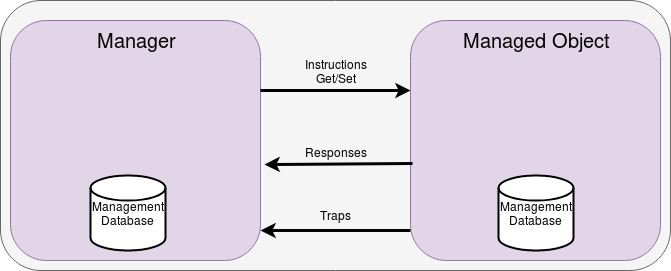
\includegraphics[width=.6\textwidth]{nm/snmp_arch}
    \caption{Architectural components of SNMP}
    \label{fig:snmp}
\end{figure}

The management database is one of the most important components of this system, because it serves as a reference to the entities that are managed in the SNMP protocol. The formal name for this database is the MIB - Management 
Information Base \cite {CITE - RFC 1155}, and its composed of a collection of objects.

\par Each object has a name, syntax and encoding \cite {CITE - RFC 1156}. The name of the object, more specifically, the \textit {Object Identifier (OID)}, is a reference to the object itself. This name is usually a 
list of integers, and they serve to build a tree-like hierarchy. This structure allows for the organization of all objects in a logical pattern, as there is a parent node, that contains references to their children, 
that provide different indexes for different objects. For human readability, there is usually a \textit {Object Descriptor}, to refer to the object type. The syntax defines the type of data structure in the object type; and 
the encoding describes how the object type is transmitted on the network. In the context of this thesis, an important group is the interfaces group, as this exposes information about the interfaces present in a system. It's OID 
is the .3.6.1.2.1.2., and contains the number of interfaces in a system, and a table containing the counters related to the interface status, like the received unicast packets, the physical address, among others. The flexibility of
the MIB allows for vendors to introduce their own databases into the MIB, while also remaining compatible with the standardized one.

\par Due to its permanence in the market, the protocol has suffered some large changes since its original design. SNMPv3 now supports important changes to the original one, most notably in the security aspects, introducing strong
authentication and encryption capabilities.

\section {Data Center Networks (DCN)}

\par The rising demand of services like music and video streaming, or mass data storage, brings an increase of demand of compute and storage infrastructures, and the shift to the cloud computing model has led to a
proliferation of large data-centers, containing thousands of physical nodes. Related to this growth is the focus on moving not only servers to a virtualised environment, by having one physical host several virtual machines and
client applications, but moving also the networking functions to a virtual environment, by replacing the dedicated network hardware with generic compute resources, in a paradigm called \textit{Network Function Virtualisation (NFV)} 
\cite {CITE - OPENSDWN}. One of the bigger gains of using NFV, is the possibility of separation of each virtual network (VN), which guarantees better performance isolation and application of Quality of Service (QoS) rules
\cite {CITE - Data center virtualisation a survey}. 
\par The design of the network architecture is central to the data-center networks, as the placement for physical hosts and virtual machines allows for sharing the resources and create a logical hierarchy of network devices. The 
study on the design of DCN has resulted in the creation of typical DC topologies, like fat-tree topologies (as seen in \ref {nm/fattree}), or others, including de Bruijn server only networks, or BCube switch heavy networks 
\cite{ popa_cost_2010 }. This approach allows for the traffic characteristics, resource consumption and costs of the networking devices be understood, so that causes for failure of this network are understood and mitigated, 
and the entire DC can run on the most optimal possible way. The organization in the DCN also allows for traffic in the network being resistant to failure scenarios, since there are multiple paths that can redirect packets 
to the correct destination, even if a link to a switch fails.

\begin{figure} [!htbp]
    \centering
    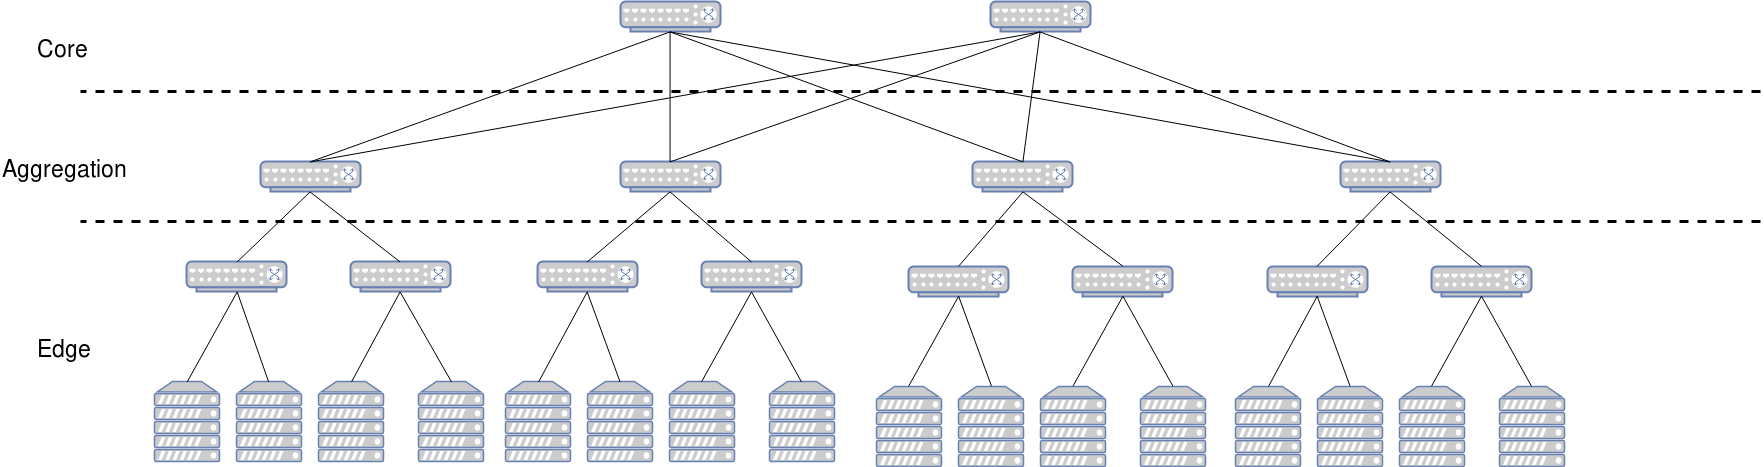
\includegraphics[width=1\textwidth]{nm/fattree}
    \caption{Visual representation of the fat tree topology commonly used in data centers}
    \label{fig:fattree}
\end{figure}

\subsection {DCN Traffic}

\par So that solutions for network management in data-centers can be developed, first there needs to an understanding of the traffic characteristics and resource allocation, and utilize this information to shape the DC fabric.
The several studies proposed in traffic engineering for traditional networks do need to be revised in DCN's, since metrics like propagation delay, can be negligible, due to the physical proximity of nodes in DC's 
\cite{CITE - data_center_virt_survey}. However, studies on DCN's have proven difficult, since many data-center operators do not wish to publish information about their applications and services. Also contributing to this fact is
the impossibility of separating the different classes of data centers, since deployments across campus, private and cloud data-centers serve different purposes and have different applications.
\par By collecting data from different types of DC's, several studies have been made about the traffic characteristics \cite{ CITE - dc_networks_chars, CITE - dc_traffic_chars, CITE - fb_datacenter}:

\begin {itemize}
    \item The placement of VMs and servers effects the bandwidth and link capacity, due to the variety of applications that can be running on the servers at any time, and this non-uniform placement of VMs contributes to higher
        amounts of traffic originating from the same rack
    \item The majority of flows \footnote {flows are sequences of packets sent from a source to a certain destination (host, anycast or multicast domain)} are described as being small in size, and short in duration,
        which are usually described as \textit {mice} flows. 
        The counterpart to these are the \textit {elephant} flows, which occupy a very large share of the bandwidth, and degrade application performance, due to choking effect to the latency-sensitive mice flows. 
        Applications are tied to the type of traffic they generate, where online gaming, VoIP and multimedia broadcasting usually originate mice flows, where the large data transfers and file-sharing originate in elephant flows. 
        However, these flows which account for 80\% of total traffic only occur less than 10\% of total flows \cite {CITE - Broadcom Engineered Elephant flow for boosting ... }.
    \item In a normal situation, link utilization is low in the layers apart from the core switches. In addition to this discovery, losses are associated with spikes in traffic, instead being related to high utilization 
        of the link, which is one of the effects of the previously mentioned elephant flows.
\end {itemize}

\subsection {DCN and SDN}

\par The centralized view that SDN controllers maintain over the networks allows for it to keep the information about the flows currently present in the network. As such, in the SDN paradigm, there is possibility to flexibly control 
the path that the packets take in the network, and improve performance of the network at a large scale. By joining the information available on DCN and SDN, the requirements for traffic engineering (TE) in SDN, from
the perspective of flow control are flow management, fault tolerance and traffic analysis \cite { CITE - traffic_engineering_sdn}. This set of four requirements set the base for properly monitoring a DCN from the 
perspective of the SDN paradigm.
\par The next section are taken from \cite { CITE - traffic_engineering_sdn}.

\subsubsection {Flow management}

Flow management refers to the capability that the controller has to set rules for packet forwarding, and maintain the low overhead that is associated with registering a new flow mod, and also limiting the amount of flow entries, 
as hardware switches usually have a set amount of flow entries that it can support. Further in this document, we explore the effect that the amount of flow entries has on OVS, where increasing the amount of flow entries also 
increases the packet loss between two hosts.
\par If we consider the fat-tree topology, then one obvious result is the fact that if one controller is responsible for the management of the entire underlying topology, then one possible results is the creation of one bottleneck
when the rules need to be deployed to a node. When the switch receives a new packet, and there are no rules to properly forward this packet, then the packet is redirected to the controller, on the form of a \textsc{PACKET\_IN} 
message, and after processing this packet a new flow mod is sent to the switch. The problem with this scenario lies in the delay that it takes between the reception of the packet, and the installation of the new
flow entry, which can be a contributing factor in packet losses in the data plane. This is an attack vector that is also explored in Distributed Denial of Service (DDoS) attacks for SDN platforms, as in an extreme scenario,
the spoofed packet addresses will not have matches on the tables, which then result on overflowing the controller \cite {early_detection_sdn_ddos}.
\par A solution for this issue is then related to decreasing the number of messages sent to the controller, by introducing some load balancing concepts. One of these concepts is related to the way that we can install the flow 
entries on the switch. The information present in the packets serve to generate the flow-match entries that are deployed on the table. To reduce the number of interactions between the controller and OF switches, then we can 
reduce the number of match fields present in the flow mods, which reduces the number of flow entries on the switch and the controller messages. Another solution is related to distribute the controller among the network, 
but keeping them connected via a separate channel.

\subsubsection {Fault tolerance} \label{sec:fault_tolerance}

Although the switches are connected in a way that are able to mitigate link, or other switch failures, in the case of faults occurring there needs to be the possibility of creation of new forwarding rules. An even bigger 
concern lies in the case when the controller fails, which will pose a larger problem in the network. For the case of node failure, fast recovery means that the OF controller can reactively react on link failures, by signaling the
switches to forward packets toward new locations; or proactively, by setting the rules prior to the occurrence of the failure. In the case that the failure is short lived, then the controller is also responsible of resetting the 
paths to the optimal state.
\par In the case of controller failover, then the backup controllers should act on this failure, and act as the new master. OF switches should connect to the set of available controllers, which should coordinate the management of 
the switch amongst themselves. After the switches first connection to the controllers, they should maintain this connection alive, but the controllers have the possibility of changing their roles. The controller roles are as follows:

\begin {itemize}
    \item \textsc {OFPCD\_ROLE\_EQUAL}, where the controller has full access to the switch, receiving all incoming messages, and can modify the state of the switch
    \item \textsc {OFPCD\_ROLE\_MASTER}, which is a similar status to the previous one, but where the switch ensures that only one switch is connected as the master role
    \item \textsc {OFPCD\_ROLE\_SLAVE} is a role that controllers has read-only access to the switch, having no permissions for altering the state of the switch. The only message that controllers registered with this role receive
        are the port-status messages
\end {itemize}

As previously mentioned, the way that controllers handle their connection is independent of the OpenFlow connection, and the failover should occur with minimal changes to the underlying flow rules and overhead.

\subsubsection {Traffic analysis}

So that the management tools can correctly display information about the state of the network, status statistics should be continuously collected and analysed. These statistics should provide the information about flows, packets
and ports, so that the measured metrics can serve as a baseline for the decisions of the controller to adapt the flow mods to enable the best possible performance. For the statistics collection there are two possible ways of 
getting the data: by continuously sampling packets from the switches; or applying sampling techniques, and generalizing the information from the sampled data \cite{CITE - low_overhead_te_elephants_detec}. The problem here lies
in the collection of the statistics in poses a problem for large scale deployments, where continuously polling the network devices introduces both overhead and very large amounts of data to be parsed, or the data is not enough
to detect failures in a short amount of time.

\section {Statistics}

\subsection {OpenFlow}

After exploring the requirements for network management, and the way the SDN model can support developing better systems, we now focus on the possibilites for obtaining this information from the networking devices. The OpenFlow 
protocol maintains a set of counters for each flow entry, port and group statistics, and this information can be queried to obtain a general view on the status of each OF switch. By sending specific controller-to-switch messages,
the switch will return a set of the maintained statistics, which can then be parsed and analysed further. 
\par Sending the port statistics message returns an array with the measured counters for each port. These counters include information like the amount of received and transmitted bytes/ packets, errors and dropped packets, and the
duration that the port is alive. 
\par The next important message is the \textsc{OFMP\_FLOW} message, since this allows for getting the individual flow statistics, and obtain the information about each flow entry, including the time that it has been set on the switch,
the number of packets/bytes in the flow, and the match fields. Also worth noting are the aggregate flow messages which describe how many packets are in the total flow entries, and also the number of flow entries that exist.
\par Also relevant is the information that is retrieved using the group statistics, as they allow to monitor the number of flows that direct to the group, and again the packet/ byte count that are matched with this group.
\par The information provided from these messages allows for a comprehensive view of the state of each switch, and a network management system (NMS) should utilize this information to achieve an understanding of the 
state of the network. 

\subsection {sFlow}

One problem arises, however, when periodic requests generate too much information, and the control channel is overflowed with messages of port statistics, which is a possible scenario when the
flow tables start getting too large. As such, a different alternative is to sample a small amount of packets from the switch, send the packet headers to the controller. One approach to this method is \textit{sFlow}, 
a standard for collection, analysis and storage of network flows and traffic, for each device and its interfaces. sFlow is implemented using embedded agents on switches and routers, which compile interface and flow samples and 
exports them to the sFlow collector via datagrams. 
\par Due to the problems that arise with continuously collecting traffic data, packet sampling has emerged as a valid solution to this problem, by collecting every \textit{n}-th packet randomly. The simplicity of the 
technique allows for reducing the complexity of sFlow agents, and having the sampling operation being done in hardware, resulting in the collection of the samples being done at the same speed of the channel it is monitoring. This
reduces the losses that are inherent to the sampling process, which leads to biased analysis of the traffic \cite {CITE - packet_sample_anomaly}.

\begin{figure} [!htbp]
    \centering
    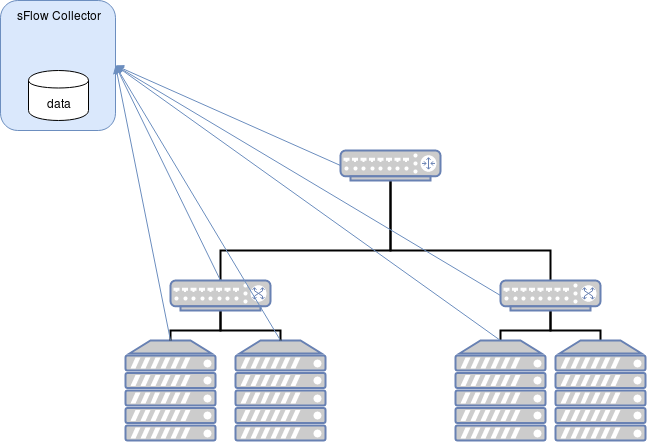
\includegraphics[width=.6\textwidth]{nm/sflow_diagram}
    \caption{Architectural components of sFlow}
    \label{fig:sflow}
\end{figure}

\par Figure \ref{fig:sflow} shows the basic architecture that composes the sFlow system. One advantage of this system is the number of systems that incorporate sFlow agents \footnote {Complete list of compliant devices: 
http://www.sflow.org/products/network.php}, allowing for a detailed analysis of flows, and enabling flexibility for scalability in the network. By utilizing a sFlow collector that can accurately collect and process the datagrams 
incoming from the Agents, this protocol can be used to control most of the central aspects in network management, like troubleshooting network problems; controlling congestion on the network; or even analysing the possible 
security threats internal and external to the network.
